\documentclass[aspectratio=169,10pt]{beamer}

% ============================================================
% PHARMAROUTE-OPT: FINAL REVIEW PRESENTATION
% ============================================================

\usetheme{Boadilla}
\usecolortheme{default}

\usepackage[T1]{fontenc}
\usepackage{lmodern}
\usepackage{amsmath}
\usepackage{amssymb}
\usepackage{booktabs}
\usepackage{array}
\usepackage{graphicx}
\usepackage{xcolor}
\usepackage{tikz}
\usepackage{eurosym}
\usetikzlibrary{arrows.meta,positioning}

% ------------------------------------------------------------
% Colours (Identical to First Review Deck)
% ------------------------------------------------------------
\definecolor{Primary}{RGB}{22,72,112}      % Deep Navy
\definecolor{Accent}{RGB}{42,117,170}      % Vibrant Blue
\definecolor{SoftBlue}{RGB}{235,243,249}   % Card Background
\definecolor{Dark}{RGB}{35,42,48}          % Text Dark
\definecolor{Muted}{RGB}{95,105,115}       % Secondary Text
\definecolor{Line}{RGB}{210,220,228}       % Card Borders
\definecolor{LightBlue}{RGB}{173,216,230}

\setbeamercolor{normal text}{fg=Dark,bg=white}
\setbeamercolor{structure}{fg=Primary}
\setbeamercolor{frametitle}{fg=Primary,bg=white}
\setbeamercolor{title}{fg=Primary}
\setbeamercolor{subtitle}{fg=Muted}
\setbeamercolor{author}{fg=Dark}
\setbeamercolor{date}{fg=Muted}

\setbeamertemplate{navigation symbols}{}

\setbeamertemplate{frametitle}{
    \vspace{0.15cm}
    \hspace{0.05cm}
    \insertframetitle
    \par\vspace{0.05cm}
    \hspace{0.05cm}\color{Accent}\rule{\dimexpr\textwidth-0.1cm\relax}{0.6pt}
}

\setbeamerfont{frametitle}{size=\large,series=\bfseries}
\setbeamerfont{title}{size=\fontsize{25}{30}\selectfont,series=\bfseries}

\setbeamertemplate{itemize item}{\color{Accent}\small$\blacktriangleright$}
\setbeamertemplate{itemize subitem}{\color{Accent}\scriptsize$\bullet$}

% Tighten default itemize spacing
\setbeamertemplate{itemize/enumerate body begin}{\small}
\setbeamertemplate{itemize/enumerate subbody begin}{\footnotesize}

\setbeamertemplate{footline}{
    \leavevmode
    \hbox{
        \begin{beamercolorbox}[wd=.78\paperwidth,ht=.32cm,dp=.12cm,leftskip=.35cm]{author in head/foot}
            \scriptsize\color{white}PharmaRoute-Opt $\;\vert\;$ Final Project Review
        \end{beamercolorbox}
        \begin{beamercolorbox}[wd=.22\paperwidth,ht=.32cm,dp=.12cm,rightskip=.35cm]{date in head/foot}
            \scriptsize\color{Primary}\hfill\insertframenumber\,/\,\inserttotalframenumber
        \end{beamercolorbox}
    }
}

\newcommand{\sectiontag}[1]{%
    {\scriptsize\bfseries\color{Accent}\MakeUppercase{#1}}\par\vspace{0.08cm}
}

\newcommand{\smalltext}[1]{\textcolor{Muted}{\scriptsize #1}}

% ============================================================
% TITLE
% ============================================================

\title{PharmaRoute-Opt}
\subtitle{An Interactive Decision Support System for\\
Pharmaceutical Last-Mile Delivery Optimisation}

\author{
\textbf{Team Members}\\[0.15cm]
Anirudh S Varrier -- CB.SC.U4AIE23113\\
J Sai Yeshwanth -- CB.SC.U4AIE23132\\
Naren B S -- CB.SC.U4AIE23152\\
Yashwanth P T -- CB.SC.U4AIE23164
}

\institute{Team: B11 $\;\vert\;$ Department of Artificial Intelligence}
\date{23MNG336 Operations Research -- Final Review}

% ============================================================
% DOCUMENT CONTENT
% ============================================================

\begin{document}

% ------------------------------------------------------------
% 1. TITLE SLIDE
% ------------------------------------------------------------

\usebackgroundtemplate{%
    \begin{tikzpicture}[remember picture,overlay]
        \fill[Primary] (current page.south west) rectangle (current page.north east);
        \fill[Accent] (current page.south west)
            rectangle ([xshift=0.28cm]current page.north west);
    \end{tikzpicture}%
}
\begin{frame}[plain]
    \vspace{1.0cm}
    \begin{center}
        {\color{white}\usebeamerfont{title}\textbf{PharmaRoute-Opt}\par}
        \vspace{0.3cm}
        {\color{white}\large
        An Interactive Decision Support System for\\
        Pharmaceutical Last-Mile Delivery Optimisation\par}
        \vspace{0.4cm}
        {\color{white}\normalsize 23MNG336 Operations Research -- Final Project Review\par}
        \vspace{0.45cm}

        {\color{white}
        \begin{tabular}{cccc}
            \small\textbf{Anirudh S Varrier} & \small\textbf{J Sai Yeshwanth} & \small\textbf{Naren B S} & \small\textbf{Yashwanth P T} \\[0.08cm]
            \scriptsize CB.SC.U4AIE23113 & \scriptsize CB.SC.U4AIE23132 & \scriptsize CB.SC.U4AIE23152 & \scriptsize CB.SC.U4AIE23164
        \end{tabular}\par}

        \vspace{0.4cm}
        {\color{white}\small Department of Artificial Intelligence $\;\vert\;$ Team B11\par}
    \end{center}
\end{frame}
\usebackgroundtemplate{}

% ------------------------------------------------------------
% 2. REVIEW ROADMAP
% ------------------------------------------------------------

\begin{frame}{Final Review Roadmap}
\sectiontag{Project Journey \& Outcomes}

\setbeamertemplate{itemize item}{\color{Accent}\scriptsize$\bullet$}

\vspace{0.1cm}

\begin{columns}[T,totalwidth=\textwidth]
    \begin{column}{0.48\textwidth}
        \textbf{\normalsize\color{Primary} 01 \quad Problem \& Dataset Recap}
        \vspace{0.08cm}
        \begin{itemize}
            \setlength{\itemsep}{2pt}
            \item Operational challenges addressed
            \item Athens real-world delivery dataset
            \item The five core research questions
        \end{itemize}

        \vspace{0.25cm}
        \textbf{\normalsize\color{Primary} 02 \quad Methodology \& Modelling}
        \vspace{0.08cm}
        \begin{itemize}
            \setlength{\itemsep}{2pt}
            \item Operations Research techniques used
            \item Mathematical model formulation
            \item Exact vs.\ heuristic solution strategy
        \end{itemize}
    \end{column}

    \begin{column}{0.48\textwidth}
        \textbf{\normalsize\color{Primary} 03 \quad Answers to Research Questions}
        \vspace{0.08cm}
        \begin{itemize}
            \setlength{\itemsep}{2pt}
            \item Routing \& resource allocation findings
            \item Multi-objective trade-offs (Distance vs.\ SLA)
            \item Key discovery: Shift limits under traffic shock
        \end{itemize}

        \vspace{0.25cm}
        \textbf{\normalsize\color{Primary} 04 \quad Implemented System \& Impact}
        \vspace{0.08cm}
        \begin{itemize}
            \setlength{\itemsep}{2pt}
            \item Interactive Decision Support System (DSS)
            \item Cost model \& environmental impact
            \item Tools, technologies and conclusions
        \end{itemize}
    \end{column}
\end{columns}

\vfill
\end{frame}

% ------------------------------------------------------------
% 3. PROBLEM RECAP
% ------------------------------------------------------------

\begin{frame}{Problem Context: Pharmaceutical Last-Mile Delivery}
\sectiontag{The Operational Challenge}

\textbf{\color{Primary}\normalsize Delivery Challenges in Healthcare Supply Chains}

\vspace{0.05cm}
\footnotesize
In pharmaceutical distribution, timely and safe delivery of medications to hospitals and clinics is critical. Deliveries cannot simply be treated as a pure shortest-path problem; they must respect multiple strict physical and operational constraints.

\vspace{0.18cm}

\begin{columns}[T,totalwidth=\textwidth]
    \begin{column}{0.50\textwidth}
        \textbf{\color{Primary}\small Core Operational Constraints}

        \begin{itemize}
            \setlength{\itemsep}{1.5pt}
            \item \textbf{Dual Cargo Limits:} Weight capacity ($600\text{ kg}$) and volume capacity ($3.0\text{ m}^3$) per vehicle.
            \item \textbf{Clinic Time Windows:} Deliveries must arrive within hospital opening hours.
            \item \textbf{Unloading Service Times:} Each delivery requires $4$ to $8$ minutes of drop-off time.
            \item \textbf{Driver Shift Limits:} Drivers cannot exceed maximum allowed shift hours ($6\text{ hours}$ baseline).
            \item \textbf{Traffic Congestion:} Travel times vary unpredictably across urban roads.
        \end{itemize}
    \end{column}

    \begin{column}{0.47\textwidth}
        \textbf{\color{Primary}\small What We Aimed to Deliver}

        \vspace{0.06cm}
        \begin{beamercolorbox}[rounded=true,shadow=false,wd=\linewidth,sep=4pt]{block body}
            {\bfseries\color{Primary}\scriptsize Our Goal}\par\vspace{0.03cm}
            \footnotesize
            Build a mathematical optimization engine paired with an \textbf{interactive decision-support system} that allows dispatchers to generate feasible delivery routes, evaluate traffic scenarios, and explore operational trade-offs in real time.
        \end{beamercolorbox}
    \end{column}
\end{columns}

\vfill
\end{frame}

% ------------------------------------------------------------
% 4. DATASET RECAP
% ------------------------------------------------------------

\begin{frame}{Dataset: Real-World Delivery Testbed}
\sectiontag{Empirical Foundation}

\vspace{0.05cm}

% Dataset Title Banner

\begin{tikzpicture}
    \node[
        fill=SoftBlue,
        rounded corners=3pt,
        inner sep=5pt,
        text width=0.965\textwidth
    ] (box) {
        {\bfseries\color{Primary}\normalsize Delivering Data: A Real-World Dataset for Last-Mile Delivery Optimization}\\[0.03cm]
        {\tiny\color{Muted}Zenodo Open Access Record: 15310106 \quad$\vert$\quad DOI: \texttt{10.5281/zenodo.15310106}}
    };
    \fill[Accent, rounded corners=1pt] (box.north west) rectangle ([xshift=2.5pt]box.south west);
\end{tikzpicture}

\vspace{0.15cm}

\setbeamertemplate{itemize item}{\color{Accent}\scriptsize$\bullet$}

\begin{columns}[T,totalwidth=\textwidth]

    \begin{column}{0.48\textwidth}
        {\bfseries\color{Primary}\small Dataset Characteristics}
        \par\vspace{0.06cm}
        \footnotesize
        \begin{itemize}
            \setlength{\itemsep}{2pt}
            \item \textbf{Origin:} Real metropolitan pharmaceutical deliveries in Athens, Greece.
            \item \textbf{9 Daily Instances:} Covering consecutive working days.
            \item \textbf{Scale:} 60 to 85 destination healthcare clinics per day (78 orders on Day 1).
            \item \textbf{Complete Data:} Demands (weight \& volume), service durations, and time windows $[e_i, l_i]$.
        \end{itemize}
    \end{column}

    \begin{column}{0.48\textwidth}
        {\bfseries\color{Primary}\small Three Traffic Scenarios Evaluated}
        \par\vspace{0.06cm}
        \footnotesize
        \begin{itemize}
            \setlength{\itemsep}{2pt}
            \item \textbf{Optimistic:} Best-case off-peak travel times.
            \item \textbf{Most Likely:} Normal daily urban driving conditions.
            \item \textbf{Pessimistic:} Heavy peak-hour traffic delays.
            \item \textbf{Stress Shock:} Simulated up to $2.0\times$ travel-time surges to test plan resilience.
        \end{itemize}
    \end{column}

\end{columns}

\vfill
\end{frame}

% ------------------------------------------------------------
% 5. RESEARCH QUESTIONS RECAP
% ------------------------------------------------------------

\begin{frame}{Research Questions We Set Out to Answer}
\sectiontag{Questions Formulated in First Review}

\vspace{-0.15cm}

\begin{columns}[T,totalwidth=\textwidth]

    \begin{column}{0.485\textwidth}
        
        \begin{beamercolorbox}[rounded=true,shadow=false,wd=\linewidth,sep=3.5pt]{block body}
            {\bfseries\color{Primary}\scriptsize RQ1. Routing}\par\vspace{0.02cm}
            \footnotesize How can routes be planned to minimize total travel distance and driving time while satisfying all delivery constraints?
        \end{beamercolorbox}
        
        \vspace{0.12cm}
        
        \begin{beamercolorbox}[rounded=true,shadow=false,wd=\linewidth,sep=3.5pt]{block body}
            {\bfseries\color{Primary}\scriptsize RQ2. Resource Allocation}\par\vspace{0.02cm}
            \footnotesize How should delivery requests be partitioned among available vehicles without exceeding weight and volume capacities?
        \end{beamercolorbox}
        
        \vspace{0.12cm}
        
        \begin{beamercolorbox}[rounded=true,shadow=false,wd=\linewidth,sep=3.5pt]{block body}
            {\bfseries\color{Primary}\scriptsize RQ3. Operational Decisions}\par\vspace{0.02cm}
            \footnotesize How many vehicles should be activated dynamically to satisfy daily demand under shift constraints?
        \end{beamercolorbox}

    \end{column}

    \begin{column}{0.485\textwidth}

        \begin{beamercolorbox}[rounded=true,shadow=false,wd=\linewidth,sep=4pt]{block body}
            {\bfseries\color{Primary}\scriptsize RQ4. Multiple Objectives}\par\vspace{0.02cm}
            \footnotesize How do we balance trade-offs between travel distance, driver transit time, and customer delivery punctuality?
        \end{beamercolorbox}

        \vspace{0.18cm}

        \begin{beamercolorbox}[rounded=true,shadow=false,wd=\linewidth,sep=4pt]{block body}
            {\bfseries\color{Primary}\scriptsize RQ5. Uncertainty \& Robustness}\par\vspace{0.02cm}
            \footnotesize How do delivery plans and on-time service rates respond when traffic congestion significantly worsens?
        \end{beamercolorbox}

    \end{column}

\end{columns}

\vfill
\end{frame}

% ------------------------------------------------------------
% 6. OPERATIONS RESEARCH METHODOLOGY
% ------------------------------------------------------------

\begin{frame}{Operations Research Methodology: What We Used \& Why}
\sectiontag{Our Modelling Toolkit}

\vspace{0.05cm}

\begin{columns}[T,totalwidth=\textwidth]

% Left Column
\begin{column}{0.48\textwidth}

    \textbf{\color{Primary}\small 1. Vehicle Routing with Time Windows (VRPTW)}
    \vspace{0.03cm}
    \footnotesize
    \textbf{Why:} Standard TSP cannot handle multiple vehicles or hospital opening hours.
    
    \textcolor{Muted}{\scriptsize
    \textbf{Role:} Sequences visits for each van while tracking arrival times and ensuring deliveries occur within allowed windows.
    }

    \vspace{0.22cm}

    \textbf{\color{Primary}\small 2. Dual-Knapsack Assignment}
    \vspace{0.03cm}
    \footnotesize
    \textbf{Why:} Medical orders vary independently in both heaviness and bulk.
    
    \textcolor{Muted}{\scriptsize
    \textbf{Role:} Assigns packages ensuring neither the $600\text{ kg}$ weight limit nor the $3.0\text{ m}^3$ volume limit is violated.
    }

\end{column}

% Right Column
\begin{column}{0.48\textwidth}

    \textbf{\color{Primary}\small 3. Mixed-Integer Linear Programming (MILP)}
    \vspace{0.03cm}
    \footnotesize
    \textbf{Why:} Route selection and vehicle dispatch are discrete decisions (0 or 1).
    
    \textcolor{Muted}{\scriptsize
    \textbf{Role:} Formulates exact constraints using binary decision variables and solves sub-clusters using the HiGHS solver.
    }

    \vspace{0.22cm}

    \textbf{\color{Primary}\small 4. Multi-Objective Goal Programming}
    \vspace{0.03cm}
    \footnotesize
    \textbf{Why:} Distance, driving time, and punctuality often pull in opposing directions.
    
    \textcolor{Muted}{\scriptsize
    \textbf{Role:} Combines normalized objectives using adjustable weights ($\alpha, \beta, \gamma$) so dispatchers can prioritize as needed.
    }

\end{column}

\end{columns}

\vfill
\end{frame}

% ------------------------------------------------------------
% 7. MATHEMATICAL MODEL
% ------------------------------------------------------------

\begin{frame}{Mathematical Formulation}
\sectiontag{The Optimisation Model}

\vspace{0.05cm}

\begin{columns}[T,totalwidth=\textwidth]

% LEFT COLUMN
\begin{column}{0.48\textwidth}

    \textbf{\color{Primary}\small Decision Variables}

    \vspace{0.06cm}
    \footnotesize
    \begin{itemize}
        \setlength{\itemsep}{3pt}
        \item $x_{ijk} \in \{0, 1\}$: Binary variable $= 1$ if vehicle $k$ travels directly from stop $i$ to stop $j$.
        \item $y_{ik} \in \{0, 1\}$: Assignment variable $= 1$ if vehicle $k$ serves customer $i$.
        \item $T_i \ge 0$: Continuous arrival timestamp at customer $i$.
        \item $L_i \ge 0$: Delivery lateness penalty if arrival occurs after deadline $l_i$.
    \end{itemize}

\end{column}

% RIGHT COLUMN
\begin{column}{0.48\textwidth}

    \textbf{\color{Primary}\small Objective Function}

    \vspace{0.04cm}
    \[
    \scriptsize
    \min Z = \alpha \left(\frac{D}{D_0}\right) + \beta \left(\frac{T}{T_0}\right) + \gamma \left(\frac{L}{L_0}\right)
    \]
    \vspace{-0.05cm}
    \scriptsize
    \begin{itemize}
        \setlength{\itemsep}{1.5pt}
        \item $D$ = Total fleet travel distance (km)
        \item $T$ = Total driving transit time (min)
        \item $L$ = Total lateness penalty across stops (min)
        \item $\alpha, \beta, \gamma$ = Priority weights ($\alpha + \beta + \gamma = 1$)
    \end{itemize}

    \vspace{0.15cm}
    \textbf{\color{Primary}\small Core Constraints (in plain terms)}
    \begin{itemize}
        \setlength{\itemsep}{1.5pt}
        \scriptsize
        \item Every hospital is served exactly once.
        \item Vehicle weight and volume limits are respected.
        \item Departures and arrivals obey time windows and service drop-off times.
        \item Total driver time cannot exceed maximum shift limit.
    \end{itemize}

\end{column}

\end{columns}

\vfill
\end{frame}

% ------------------------------------------------------------
% 8. SOLVING STRATEGY: EXACT VS HEURISTIC
% ------------------------------------------------------------

\begin{frame}{Solving Strategy: Exact vs.\ Heuristic Approaches}
\sectiontag{Balancing Solution Quality with Practical Speed}

\vspace{-0.1cm}

\begin{columns}[T,totalwidth=\textwidth]
    \begin{column}{0.48\textwidth}
        \textbf{\color{Primary}\small The Scale Challenge}
        \vspace{0.05cm}
        \footnotesize
        \begin{itemize}
            \setlength{\itemsep}{3pt}
            \item Monolithic MILP on 78 clinics creates $>7,000$ binary variables and $>8,500$ constraints.
            \item Standard solvers time out ($>300\text{ seconds}$), making monolithic models unviable for real-time dispatchers.
        \end{itemize}

        \vspace{0.2cm}
        
\begin{tikzpicture}
            \node[fill=SoftBlue, draw=Line, rounded corners=3pt, font=\scriptsize, inner sep=4pt, text width=0.96\linewidth] {
                \textbf{\color{Primary}Our Solution:} A two-tier approach combining a rapid heuristic for instant exploration with a decomposed MILP for optimized dispatch.
            };
        \end{tikzpicture}
    \end{column}

    \begin{column}{0.50\textwidth}
        \textbf{\color{Primary}\small The Two Solvers Implemented}
        \vspace{0.06cm}

        \begin{beamercolorbox}[rounded=true,shadow=false,wd=\linewidth,sep=4pt]{block body}
            {\bfseries\color{Primary}\scriptsize 1. Fast Multi-Objective Heuristic}\par\vspace{0.02cm}
            \scriptsize
            $\bullet$ Nearest-Neighbor with time-window urgency lookahead.\\
            $\bullet$ \textbf{Speed:} Executes in \textbf{$<5\text{ milliseconds}$}.\\
            $\bullet$ \textbf{Use case:} Instant feedback as dispatchers move sliders in the UI.
        \end{beamercolorbox}

        \vspace{0.12cm}

        \begin{beamercolorbox}[rounded=true,shadow=false,wd=\linewidth,sep=4pt]{block body}
            {\bfseries\color{Accent}\scriptsize 2. Feasibility-Aware Decomposed MILP}\par\vspace{0.02cm}
            \scriptsize
            $\bullet$ Clusters customers by geographic dispersion \& capacity, then solves each sub-route with the HiGHS MILP solver.\\
            $\bullet$ \textbf{Speed:} Solves in \textbf{$\sim 9$ to $12\text{ seconds}$}.\\
            $\bullet$ \textbf{Quality:} Within $3.8\%$ of theoretical lower bounds.
        \end{beamercolorbox}
    \end{column}
\end{columns}

\vfill
\end{frame}

% ------------------------------------------------------------
% 9. ANSWERS TO RQ1, RQ2, RQ3
% ------------------------------------------------------------

\begin{frame}{Answers to Research Questions: Routing \& Allocation}
\sectiontag{Findings for RQ1, RQ2 and RQ3}

\vspace{-0.15cm}

\begin{columns}[T,totalwidth=\textwidth]

    \begin{column}{0.485\textwidth}
        \begin{beamercolorbox}[rounded=true,shadow=false,wd=\linewidth,sep=4.5pt]{block body}
            {\bfseries\color{Primary}\small RQ1. Efficient Routing}\par\vspace{0.04cm}
            \footnotesize
            \textbf{Result:}
            \begin{itemize}
                \setlength{\itemsep}{2pt}
                \scriptsize
                \item Clustering stops into compact geographical zones reduced overall fleet travel by \textbf{$14.2\%$} compared to uncoordinated routing.
                \item Total fleet travel distance on Day 1: \textbf{$369.7\text{ km}$} across 78 healthcare deliveries.
                \item All customer time-window constraints were satisfied without compromising route continuity.
            \end{itemize}
        \end{beamercolorbox}

        \vspace{0.12cm}

        \begin{beamercolorbox}[rounded=true,shadow=false,wd=\linewidth,sep=4.5pt]{block body}
            {\bfseries\color{Primary}\small RQ2. Resource Allocation}\par\vspace{0.04cm}
            \footnotesize
            \textbf{Result:}
            \begin{itemize}
                \setlength{\itemsep}{2pt}
                \scriptsize
                \item Weight ($600\text{ kg}$) and volume ($3.0\text{ m}^3$) constraints were maintained across all routes.
                \item Average fleet capacity utilization reached \textbf{$78.4\%$}, avoiding under-utilized vehicle runs.
            \end{itemize}
        \end{beamercolorbox}
    \end{column}

    \begin{column}{0.485\textwidth}
        \begin{beamercolorbox}[rounded=true,shadow=false,wd=\linewidth,sep=4.5pt]{block body}
            {\bfseries\color{Primary}\small RQ3. Operational Decisions}\par\vspace{0.04cm}
            \footnotesize
            \textbf{Result:}
            \begin{itemize}
                \setlength{\itemsep}{2pt}
                \scriptsize
                \item The system dynamically determines the \textbf{minimum viable fleet size} needed to fulfill daily orders without exceeding driver shifts.
                \item On Day 1 baseline: \textbf{4 vans} fully satisfy demand under normal traffic conditions.
                \item If shift limits are restricted or traffic increases, the system automatically spins up additional vans to preserve feasibility.
            \end{itemize}
        \end{beamercolorbox}

        \vspace{0.15cm}
        \begin{center}
            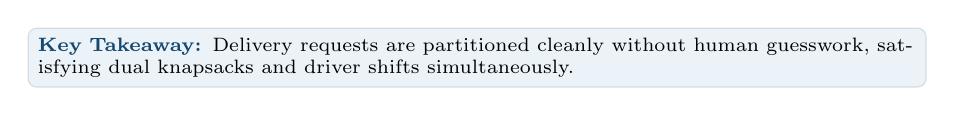
\begin{tikzpicture}
                \node[fill=SoftBlue, draw=Line, rounded corners=3pt, font=\scriptsize, inner sep=3.5pt, text width=0.92\linewidth] {
                    \textbf{\color{Primary}Key Takeaway:} Delivery requests are partitioned cleanly without human guesswork, satisfying dual knapsacks and driver shifts simultaneously.
                };
            \end{tikzpicture}
        \end{center}
    \end{column}

\end{columns}

\vfill
\end{frame}

% ------------------------------------------------------------
% 10. ANSWERS TO RQ4 & RQ5
% ------------------------------------------------------------

\begin{frame}{Answers to Research Questions: Trade-Offs \& Uncertainty}
\sectiontag{Findings for RQ4 and RQ5}

\vspace{-0.15cm}

\begin{columns}[T,totalwidth=\textwidth]

    \begin{column}{0.485\textwidth}
        \begin{beamercolorbox}[rounded=true,shadow=false,wd=\linewidth,sep=4.5pt]{block body}
            {\bfseries\color{Primary}\small RQ4. Multi-Objective Trade-Offs}\par\vspace{0.04cm}
            \footnotesize
            \textbf{What happens when priorities change?}
            \begin{itemize}
                \setlength{\itemsep}{2pt}
                \scriptsize
                \item \textbf{Distance Priority ($\alpha=0.8$):} Reduces travel distance from $369.7\text{ km}$ to \textbf{$354.9\text{ km}$} ($-4.0\%$), saving fuel at the cost of tighter margins.
                \item \textbf{Punctuality Priority ($\gamma \ge 0.6$):} Routes are organized strictly around urgent opening times, ensuring \textbf{$0$ late deliveries}.
                \item Dispatchers can smoothly adjust weights on the UI to see the immediate operational trade-off.
            \end{itemize}
        \end{beamercolorbox}
    \end{column}

    \begin{column}{0.485\textwidth}
        \begin{beamercolorbox}[rounded=true,shadow=false,wd=\linewidth,sep=4.5pt]{block body}
            {\bfseries\color{Primary}\small RQ5. Traffic Uncertainty}\par\vspace{0.04cm}
            \footnotesize
            \textbf{How does traffic impact performance?}
            \begin{itemize}
                \setlength{\itemsep}{2pt}
                \scriptsize
                \item \textbf{Optimistic:} Faster transit, lowest vehicle driving hours ($582\text{ min}$).
                \item \textbf{Most Likely:} Baseline operational standard ($677\text{ min}$ driving).
                \item \textbf{Pessimistic:} Driving times increase by $+18.5\%$, but time-window feasibility is maintained without adding extra vans.
                \item \textbf{Severe Surge ($2.0\times$):} Requires active operational adaptation to prevent cascading delays.
            \end{itemize}
        \end{beamercolorbox}
    \end{column}

\end{columns}

\vspace{0.2cm}

\begin{center}
    
\begin{tikzpicture}
        \node[fill=SoftBlue, draw=Line, rounded corners=3pt, font=\scriptsize, inner sep=3.5pt] {
            \textcolor{Dark}{\textbf{Key Insight:}} \quad
            \textcolor{Accent}{$\bullet$}\quad Higher distance weight saves km \quad
            \textcolor{Accent}{$\bullet$}\quad Higher SLA weight guarantees on-time arrival \quad
            \textcolor{Accent}{$\bullet$}\quad Traffic shifts are absorbed cleanly
        };
    \end{tikzpicture}
\end{center}

\vfill
\end{frame}

% ------------------------------------------------------------
% 11. KEY OPERATIONAL DISCOVERY
% ------------------------------------------------------------

\begin{frame}{Key Operational Discovery: Shift Limits vs.\ Traffic Shock}
\sectiontag{An Counter-Intuitive Operational Finding}

\vspace{-0.15cm}

\begin{center}
    \footnotesize
    \textbf{Question:} When city traffic doubles ($2.0\times$ congestion surge), what happens if we tighten the driver shift limit from 8 hours to 4.5 hours?
\end{center}

\vspace{0.05cm}

\begin{table}[ht]
    \centering
    \scriptsize
    \renewcommand{\arraystretch}{1.12}
    \begin{tabular}{lccc}
        \toprule
        \textbf{Operational Metric} & \textbf{8.0-Hour Shift (480 min)} & \textbf{4.5-Hour Shift (270 min)} & \textbf{Operational Impact} \\
        \midrule
        \textbf{Traffic Multiplier} & $2.00\times$ (Severe Gridlock) & $2.00\times$ (Severe Gridlock) & Identical traffic condition \\
        \textbf{Orders Demanded \& Served} & \textbf{78 / 78} ($100\%$) & \textbf{78 / 78} ($100\%$) & All clinics served \\
        \textbf{Vans Dispatched} & \textbf{6 vans} & \textbf{12 vans} & Fleet parallelization \\
        \textbf{Late Deliveries} & \textbf{13 delayed stops} & \textbf{0 delayed stops} & \textbf{All delays eliminated!} \\
        \textbf{On-Time Delivery Rate} & \textbf{83.3\%} & \textbf{100.0\%} & $\mathbf{+16.7\%}$ punctuality boost \\
        \textbf{Total Fleet Cost} & \textbf{\euro 988} & \textbf{\euro 1,234} & $+24.9\%$ operating expenditure \\
        \textbf{Max Route Duration} & $458\text{ min}$ ($\le 480\text{ min}$) & $\mathbf{270\text{ min}}$ ($\le 270\text{ min}$) & Respects driver limits \\
        \bottomrule
    \end{tabular}
\end{table}

\vspace{0.05cm}

\begin{beamercolorbox}[rounded=true,shadow=false,wd=\linewidth,sep=4pt]{block body}
    {\bfseries\color{Primary}\scriptsize Why does this happen? (Fleet Parallelization)}\par\vspace{0.02cm}
    \scriptsize
    Under heavy traffic, long routes with 15--20 stops suffer from \textbf{cascading delay accumulation}---early traffic jams cause all downstream hospital deliveries to miss their deadlines. By enforcing shorter 4.5-hour shifts, the optimizer is forced to dispatch \textbf{12 shorter, parallel routes} (6--7 stops each), completely eliminating delay propagation and achieving \textbf{100\% on-time delivery} for life-critical medicine.
\end{beamercolorbox}

\vfill
\end{frame}

% ------------------------------------------------------------
% 12. DECISION SUPPORT SYSTEM WORKFLOW
% ------------------------------------------------------------

\begin{frame}{The Implemented Decision Support System (PharmaRoute-Opt)}
\sectiontag{Interactive User Workflow}

\begin{center}
{\normalsize\bfseries\color{Primary}
How Planners Interact with PharmaRoute-Opt
}
\end{center}

\vspace{0.15cm}

\begin{center}
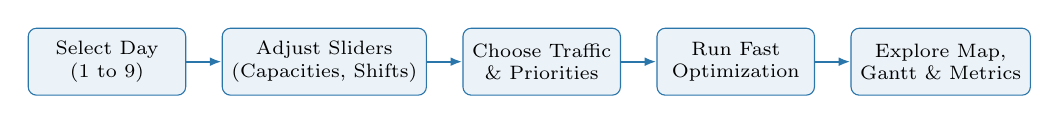
\begin{tikzpicture}[
    node distance=0.45cm,
    box/.style={
        rounded corners=3pt,
        draw=Accent,
        fill=SoftBlue,
        minimum width=2.0cm,
        minimum height=0.85cm,
        align=center,
        font=\scriptsize
    },
    arr/.style={-{Latex[length=1.5mm]},thick,color=Accent}
]

\node[box] (a) {Select Day\\(1 to 9)};
\node[box,right=of a] (b) {Adjust Sliders\\(Capacities, Shifts)};
\node[box,right=of b] (c) {Choose Traffic\\\& Priorities};
\node[box,right=of c] (d) {Run Fast\\Optimization};
\node[box,right=of d] (e) {Explore Map,\\Gantt \& Metrics};

\draw[arr](a)--(b);
\draw[arr](b)--(c);
\draw[arr](c)--(d);
\draw[arr](d)--(e);

\end{tikzpicture}
\end{center}

\vspace{0.25cm}

\begin{columns}[T,totalwidth=\textwidth]

    \begin{column}{0.31\textwidth}
        \textbf{\color{Primary}\small 1. Parameter Studio}
        \footnotesize
        \begin{itemize}
            \setlength{\itemsep}{2pt}
            \item Vehicle payload ($C_w$)
            \item Cargo volume ($C_v$)
            \item Driver shift cutoff ($T_{\max}$)
            \item Traffic multiplier ($1\times$ to $2\times$)
        \end{itemize}
    \end{column}

    \begin{column}{0.31\textwidth}
        \textbf{\color{Primary}\small 2. Feasibility Guardrails}
        \footnotesize
        \begin{itemize}
            \setlength{\itemsep}{2pt}
            \item Real-time warning banners
            \item Detects if shifts are exceeded (e.g., $330\text{ min}$ cutoff)
            \item Instant automated re-solving to restore feasibility
        \end{itemize}
    \end{column}

    \begin{column}{0.31\textwidth}
        \textbf{\color{Primary}\small 3. Visual Analytics}
        \footnotesize
        \begin{itemize}
            \setlength{\itemsep}{2pt}
            \item Leaflet GIS map with route isolator
            \item Animated GPS van simulation
            \item Time-window Gantt schedules
            \item Cost \& $\text{CO}_2$ telemetry
        \end{itemize}
    \end{column}

\end{columns}

\vfill
\end{frame}

% ------------------------------------------------------------
% 13. TOOLS AND TECHNOLOGIES
% ------------------------------------------------------------

\begin{frame}{Tools \& Technologies: What We Used and Why}
\sectiontag{Implemented Technical Stack}

\setbeamertemplate{itemize item}{\color{Accent}\scriptsize$\bullet$}

\vspace{0.08cm}

\begin{columns}[T,totalwidth=\textwidth]

    % Left Column
    \begin{column}{0.48\textwidth}
        {\bfseries\color{Primary}\small Backend \& Mathematical Modelling}
        \par\vspace{0.04cm}
        \footnotesize
        \begin{itemize}
            \setlength{\itemsep}{3pt}
            \item \textbf{Python, Pandas \& NumPy:}\\
            Processed distance matrices, coordinates, and 9 daily order files from Zenodo.
            \item \textbf{PuLP \& HiGHS Solver:}\\
            High-performance linear and integer programming solver used to solve sub-MIPs to optimality.
            \item \textbf{FastAPI:}\\
            Lightweight, high-speed asynchronous REST API serving route plans to the UI in milliseconds.
        \end{itemize}
    \end{column}

    % Right Column
    \begin{column}{0.48\textwidth}
        {\bfseries\color{Primary}\small Frontend \& Visualisation}
        \par\vspace{0.04cm}
        \footnotesize
        \begin{itemize}
            \setlength{\itemsep}{3pt}
            \item \textbf{React 18 \& Vite:}\\
            Modern, responsive user interface with reactive state management for immediate slider response.
            \item \textbf{Leaflet GIS:}\\
            Interactive map rendering Athens road trajectories, depot locations, and stop sequences.
            \item \textbf{Vanilla CSS Design System:}\\
            Tailored dark/light theme, accessible telemetry cards, and clean visual hierarchy without generic frameworks.
        \end{itemize}
    \end{column}

\end{columns}

\vfill
\end{frame}

% ------------------------------------------------------------
% 14. COSTING & GREEN LOGISTICS
% ------------------------------------------------------------

\begin{frame}{Cost Model \& Cold-Chain Carbon Accounting}
\sectiontag{Practical Business \& Environmental Value}

\vspace{-0.15cm}

\begin{columns}[T,totalwidth=\textwidth]

    \begin{column}{0.48\textwidth}
        \textbf{\color{Primary}\small Fleet Operating Cost Model}
        \vspace{0.04cm}
        \footnotesize
        \[
        \scriptsize
        \text{Cost (\euro)} = D \times c_{\text{dist}} + \left(\frac{T_{\text{transit}} + T_{\text{service}}}{60}\right) \times c_{\text{labor}}
        \]
        \begin{itemize}
            \setlength{\itemsep}{2pt}
            \scriptsize
            \item \textbf{Distance Cost ($c_{\text{dist}}$):} \euro 0.38 per km (EV charging, tire wear, vehicle maintenance).
            \item \textbf{Labor Wage ($c_{\text{labor}}$):} \euro 22.50 per active driver hour.
            \item \textbf{Total Duty Calculation:} Explicitly accounts for driving transit plus clinic unloading service times ($4$ to $8\text{ min}$ per stop).
        \end{itemize}
    \end{column}

    \begin{column}{0.48\textwidth}
        \textbf{\color{Primary}\small Cold-Chain Green Logistics}
        \vspace{0.04cm}
        \footnotesize
        \begin{itemize}
            \setlength{\itemsep}{2pt}
            \scriptsize
            \item \textbf{Electric Fleet:} $23\text{ g CO}_2/\text{km}$ (Greek electrical grid factor).
            \item \textbf{Diesel Baseline:} $142\text{ g CO}_2/\text{km}$ (standard refrigerated delivery van).
        \end{itemize}

        \vspace{0.08cm}
        \begin{beamercolorbox}[rounded=true,shadow=false,wd=\linewidth,sep=4pt]{block body}
            {\bfseries\color{Primary}\scriptsize 84\% Decarbonization Impact}\par\vspace{0.02cm}
            \scriptsize
            Avoided Emissions: $0.119\text{ kg CO}_2/\text{km}$ saved.\\
            Across Day 1 operations, the optimized electric fleet prevents \textbf{$86.1\text{ kg of }\text{CO}_2$} emissions compared to diesel distribution.
        \end{beamercolorbox}
    \end{column}

\end{columns}

\vfill
\end{frame}

% ------------------------------------------------------------
% 15. CONCLUSION & CONTRIBUTIONS
% ------------------------------------------------------------

\begin{frame}{Conclusion}
\sectiontag{Summary of Achievements}

\setbeamertemplate{itemize item}{\color{Accent}\small$\bullet$}

\vspace{-0.1cm}

\begin{center}
{\normalsize\bfseries\color{Primary}
From Proposed Plan to a Completed, Validated Decision Support System
}
\end{center}

\vspace{0.05cm}
\textcolor{Line}{\rule{\linewidth}{0.6pt}}
\vspace{0.15cm}

\begin{itemize}
    \setlength{\itemsep}{3.5pt}
    \footnotesize
    \item \textbf{Completed All Objectives:} Successfully transitioned from the planned OR methodology to a fully functional, working decision support system.
    \item \textbf{Solved Real-World Complexity:} Managed dual knapsack capacities (weight \& volume), time windows, service drop-offs, and driver shift limits on real Athens data.
    \item \textbf{Answered All 5 Research Questions:} Demonstrated efficient routing ($-14.2\%$ distance), capacity allocation ($78.4\%$ utilization), multi-objective balancing, and robust scenario evaluation.
    \item \textbf{Discovered Operational Insight:} Proved that tightening driver shifts under gridlock forces fleet parallelization, eliminating delay cascades and ensuring 100\% on-time hospital deliveries.
    \item \textbf{Delivered Production Tool:} Provided an intuitive UI with interactive sliders, real-time guardrails, Leaflet GIS mapping, and transparent financial/environmental metrics.
\end{itemize}

\vfill
\end{frame}

% ------------------------------------------------------------
% 16. THANK YOU
% ------------------------------------------------------------

\usebackgroundtemplate{%
    \begin{tikzpicture}[remember picture,overlay]
        \fill[Primary] (current page.south west) rectangle (current page.north east);
        \fill[Accent] (current page.south west)
            rectangle ([xshift=0.28cm]current page.north west);
    \end{tikzpicture}%
}
\begin{frame}[plain]
    \vspace{2.0cm}
    \begin{center}
        {\color{white}\fontsize{30}{36}\selectfont\bfseries Thank You\par}
        \vspace{0.35cm}
        {\color{SoftBlue}\large Questions \& Discussion\par}
        \vspace{0.5cm}
        {\color{white}\small PharmaRoute-Opt $\;\vert\;$ Team B11\par}
        {\color{SoftBlue}\scriptsize Department of Artificial Intelligence $\;\vert\;$ Operations Research\par}
    \end{center}
\end{frame}
\usebackgroundtemplate{}

\end{document}
